\QuoteDirectNoPage{GNU Privacy Guard}{gnupghp} ist eine vollständige und freie Implementierung des OpenPGP Standards, der in RFC 4880 \RefIt{rfc4880} definiert ist.

Es handelt hier sich um ein Verschlüsselungsverfahren, das asymmetrische Public-Key Verfahren mit symmetrischen Verfahren kombiniert \QuoteIndirect{rfc4880}{S. 1}.

Ein symmetrisches Verschlüsselungsverfahren benutzt nur einen einzigen Schlüssel für das Verschlüsseln und Entschlüsseln. Dieser muss also beiden Kommunikationspartnern zur Verfügung stehen, darf aber niemand anderem zugänglich sein. Die Übertragung eines solchen Schlüssels wird deshalb häufig über ein asymmetrisches Verschlüsselungsverfahren bewerkstelligt.
% toref

Ein asymmetrisches Public-Key Verfahren besteht auf Sender -und Empfänger-Seite jeweils aus einem Schlüsselpaar. Dieses setzt sich aus einem öffentlichen und einem privaten Schlüssel zusammen, die gemeinsam generiert werden. Nur die öffentlichen Schlüssel werden ausgetauscht und erlauben der jeweils anderen Partei für den Besitzer des Schlüsselpaars zu verschlüsseln. Der private Schlüssel wird vom Besitzer zum Entschlüsseln benutzt und kann mit einem Passwort geschützt sein.
% toref

\begin{figure}[htb]
	%\Centerfloat
	\centering
	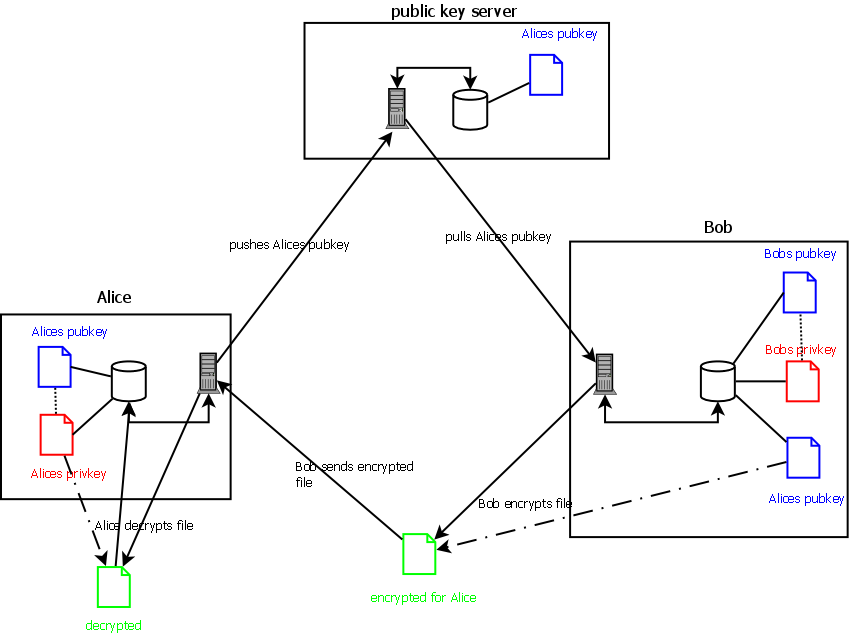
\includegraphics[scale=0.4]{Content/Problematik/BetrachtungDatenschutz/Verschluesselung/asymcrypto.png}
	\caption{Asymmetrisches Verschlüsselungsverfahren in der Praxis}
	\label{fig:asymcrypto}
\end{figure}

\autoref{fig:asymcrypto} stellt schematisch einen vereinfachten Ablauf einer verschlüsselten einseitigen Kommunikation von Bob zu Alice dar, basierend auf dem asymmetrischen Verschlüsselungsverfahren. Beide Parteien benötigen zunächst ein Schlüsselpaar, welches lokal generiert wird. Danach müssen die Parteien die benötigten öffentlichen Schlüssel austauschen. Dies kann manuell oder über einen öffentlichen Server geschehen. Als nächsten Schritt benutzt Bob den öffentlichen Schlüssel von Alice, um die Nachricht für Alice zu verschlüsseln. Dann verschlüsselt und sendet er diese. Anschließend benutzt Alice ihren privaten Schlüssel um die Nachricht zu entschlüsseln. \QuoteIndirect{Ferguson:2003:PC:862106}{Kapitel 3.3}

Hierbei kommt die Frage auf, woher Bob weiß, dass er den korrekten öffentlichen Schlüssel von Alice besitzt, wenn er diesen über einen öffentlichen Server geladen hat. Um dies festzustellen, wird ein \QuoteM{Secure Hash Algorithm} benutzt, der gewissermaßen den Fingerabdruck des öffentlichen Schlüssels darstellt. Bob kann nun Alice über einen sicheren Kanal kontaktieren (z.B. persönlich) und fragen, ob ihr Fingerabdruck des öffentlichen Schlüssels dem entspricht, den er lokal sieht. Aufgrund der Kollisionsunwahrscheinlichkeit von z.B. SHA-1 erlaubt dies eine sinnvolle Aussage über die Echtheit des öffentlichen Schlüssels, den Bob heruntergeladen hat. \QuoteIndirect{Ferguson:2003:PC:862106}{Kapitel 6.2.2}

GPG ist im Ablauf also ähnlich wie \autoref{fig:asymcrypto}, benutzt allerdings auch das symmetrische Verschlüsselungsverfahren in dem Verschlüsselungsprozess. Beim Sender wird dabei die Nachricht selbst lediglich über das symmetrische Verfahren mit einem einmaligen \QuoteM{session key} verschlüsselt. Dieser \QuoteM{session key} wird dann mit dem öffentlichen Schlüssel des Empfängers über das asymmetrische Verschlüsselungsverfahren verschlüsselt. Der symmetrische Schlüssel wird dann am Anfang der Nachricht mitgeschickt. Der Empfänger muss dann erst mit seinem privaten Schlüssel den \QuoteM{session key} entschlüsseln und dann mit diesem die eigentliche Nachricht. Dies geschieht natürlich auf Programmebene und wird nicht manuell vom Benutzer durchgeführt. \QuoteIndirect{rfc4880}{S. 6}

Anzumerken ist, dass GPG nicht nur für Verschlüsselung, sondern auch für Signierung benutzt werden kann. Damit kann der Absender einer Nachricht kryptografisch verifiziert werden. \QuoteIndirect{rfc4880}{S. 7}

GPG wird in der Praxis vielfältig benutzt. Dazu gehört das manuelle Verschlüsseln von Dateien für Andere, das Signieren von \QuoteM{git commits}
und das Verschlüsseln des Nachrichteninhaltes einer E-Mail.

Angenommen, die E-Mail selber ist über das SMTP Protokoll in sicherer Weise weitergeleitet worden, ohne dass ein Dritter diese verändern oder sehen konnte. Wenn die E-Mail auf dem Zielserver eintrifft, liegt sie dort dennoch als Klartext vor und wird durch die verschiedenen Komponenten innerhalb des Servers durchgereicht. Ist der E-Mail Server kompromittiert, so ist auch die Nachricht kompromittiert. Ist die Nachricht allerdings GPG-verschlüsselt, so ist dies nicht der Fall. Zumindest nicht für den Body.
